\documentclass[aps,prapplied,reprint,groupedaddress,twocolumn,superscriptaddress,linenumbers]{revtex4-2}
\usepackage{CJK}

\usepackage{graphicx}
\usepackage{dcolumn}
\usepackage{bm}
\usepackage{amsmath}
\usepackage{siunitx}
\usepackage{enumitem}
\usepackage{booktabs}

\begin{document}

\preprint{}

\title{Quantum-referenced refractive-index calibration of air at 1762 nm for environmental phase compensation in quantum optical interfaces}

\author{Wei Wu}
\affiliation{Albert-Ludwigs-Universität Freiburg, Physikalisches Institut, Hermann-Herder-Straße 3, 79104 Freiburg, Germany}
\affiliation{EUCOR Centre for Quantum Science and Quantum Computing, University of Freiburg, Hermann-Herder-Straße 3, 79104 Freiburg, Germany}
\author{Tobias Sch{\"a}tz}
\affiliation{Albert-Ludwigs-Universität Freiburg, Physikalisches Institut, Hermann-Herder-Straße 3, 79104 Freiburg, Germany}
\affiliation{EUCOR Centre for Quantum Science and Quantum Computing, University of Freiburg, Hermann-Herder-Straße 3, 79104 Freiburg, Germany}
\author{Ulrich Warring}
\affiliation{Albert-Ludwigs-Universität Freiburg, Physikalisches Institut, Hermann-Herder-Straße 3, 79104 Freiburg, Germany}

\date{\today}

\begin{abstract}
Free-space optical paths in quantum computing and networking platforms accumulate phase errors from environmentally driven refractive-index fluctuations. Existing refractivity models, designed for visible and near-infrared wavelengths, lack experimental validation at atomic clock transition wavelengths, particularly those in the telecommunications-compatible regime used in trapped-ion platforms. Here we report a quantum-referenced experimental calibration of the refractive index of air at \SI{1762}{\nano\meter}, the clock transition wavelength of $^{138}\mathrm{Ba}^+$. Over an eight-month measurement campaign, a dual-wavelength Michelson interferometer illuminated by a \SI{1762}{\nano\meter} probe laser referenced to a single trapped ion recorded differential phase accumulation alongside co-located environmental sensors. The measured temperature and pressure coefficients agree with the Mathar model to within \SI{0.35}{\percent} and \SI{0.93}{\percent}, respectively, when the model is evaluated on the identical environmental conditions. The humidity coefficient differs from the same-condition Mathar surrogate by \SI{24.8}{\percent} in the direction opposite to a resonance-enhancement prediction; the difference is fully covered by the humidity-sensor gain systematic and is reported as unresolved pending independent sensor calibration. For a representative \SI{1}{\meter} free-space path under diurnal environmental swings, a single baseline calibration removes the static offset of \SI{4.16}{\radian} per meter that dominates the raw Mathar residual, after which feed-forward compensation using the measured coefficients reduces the residual phase error by approximately \SI{5}{\percent} compared to the debiased Mathar model. The open dataset of \num{145784} synchronized measurements constitutes the first long-duration, atom-frequency-referenced refractivity benchmark at \SI{1762}{\nano\meter}, relevant to phase-stable quantum networks, precision optical metrology, and atmospheric sensing.
\end{abstract}

\maketitle

\section{Introduction}
\label{sec:intro}

Optical interconnects between remote trapped-ion quantum nodes require phase-stable links for protocols that depend on the first-order coherence of the optical fields, such as free-space optical clock comparisons \cite{giorgetta2013optical,shen2022free} and coherent detection of transmitted fields. Photon-counting protocols based on post-selection, such as atomic-ensemble quantum memories \cite{duan2001long} and Barrett-Kok-type schemes \cite{barrett2005efficient}, are insensitive to the common optical phase accumulated along the link and therefore do not require phase-stable optical paths. For $^{138}\mathrm{Ba}^+$ based quantum networks requiring phase-stable links, the operating wavelength is \SI{1762}{\nano\meter}, where the $6S_{1/2} \rightarrow 5D_{5/2}$ electric quadrupole transition provides the physical two-level system \cite{dietrich2009barium,arnold2020precision}. A central challenge is that environmental fluctuations like temperature ($T$), humidity ($H$), and pressure ($P$), affect the refractive index ($n$) along the optical path and induce phase errors that must be considered to preserve operational fidelities.

Compensation requires accurate knowledge of the refractive index's environmental dependence at the operating wavelength. Generalized atmospheric refractivity formulations, such as the Edl\'{e}n, Ciddor, and Mathar models, provide predictions across the visible and near-infrared \cite{edlen1966refractive,ciddor1996refractive,mathar2007refractive}. However, these models rely on refractive index data at a sparse set of calibration wavelengths and interpolate between them via dispersion formulas. Moreover, the Edl\'{e}n and Ciddor formulations were empirically calibrated over the visible and near-infrared (\SIrange{0.4}{1.3}{\micro\meter}), and their stated validity does not extend beyond the \SI{1.7}{\micro\meter} telecommunications window, leaving the $^{138}\mathrm{Ba}^+$ clock transition at \SI{1762}{\nano\meter} outside the calibrated range. The Mathar model generalizes the Ciddor dispersion formalism into the mid-infrared and is currently used to cover the wavelength regime of \SI{1762}{\nano\meter}, but it retains the averaged broadband character of its predecessors. These generic models inherently miss wavelength-specific features near molecular absorption lines, where anomalous dispersion modifies the sensitivity of refractive index to the absorbing species' partial pressure \cite{hobbs2000introduction}. At \SI{1762}{\nano\meter}, this concern is relevant since the wavelength lies between adjacent water-vapor absorption lines \cite{gordon2022hitran2020}, where dispersion may deviate from the broadband average. No direct refractivity measurement at this wavelength has been reported, to our knowledge, leaving the accuracy of existing models unvalidated for $^{138}\mathrm{Ba}^+$ quantum network applications. This motivates an empirical calibration of the environmental response at this wavelength, which we address in this work.

Here we report a direct calibration of the refractive index of air at \SI{1762}{\nano\meter} over an eight-month measurement campaign, yielding environmental coefficients $\partial n/\partial X$ ($X = T, H, P$). Comparing the measured coefficients with the Mathar model on identical environmental conditions, we find agreement within \SI{0.35}{\percent} and \SI{0.93}{\percent} for temperature and pressure, respectively, while the humidity coefficient differs by \SI{24.8}{\percent} in the direction opposite to a resonance-enhancement prediction; this difference is fully covered by the humidity-sensor gain systematic and is reported as unresolved pending independent sensor calibration. The results provide the first direct experimental benchmark of the Mathar model at a quantum clock transition wavelength, with implications for feed-forward phase compensation in free-space quantum links and for precision optical metrology.

\begin{figure}[htbp]
\centering
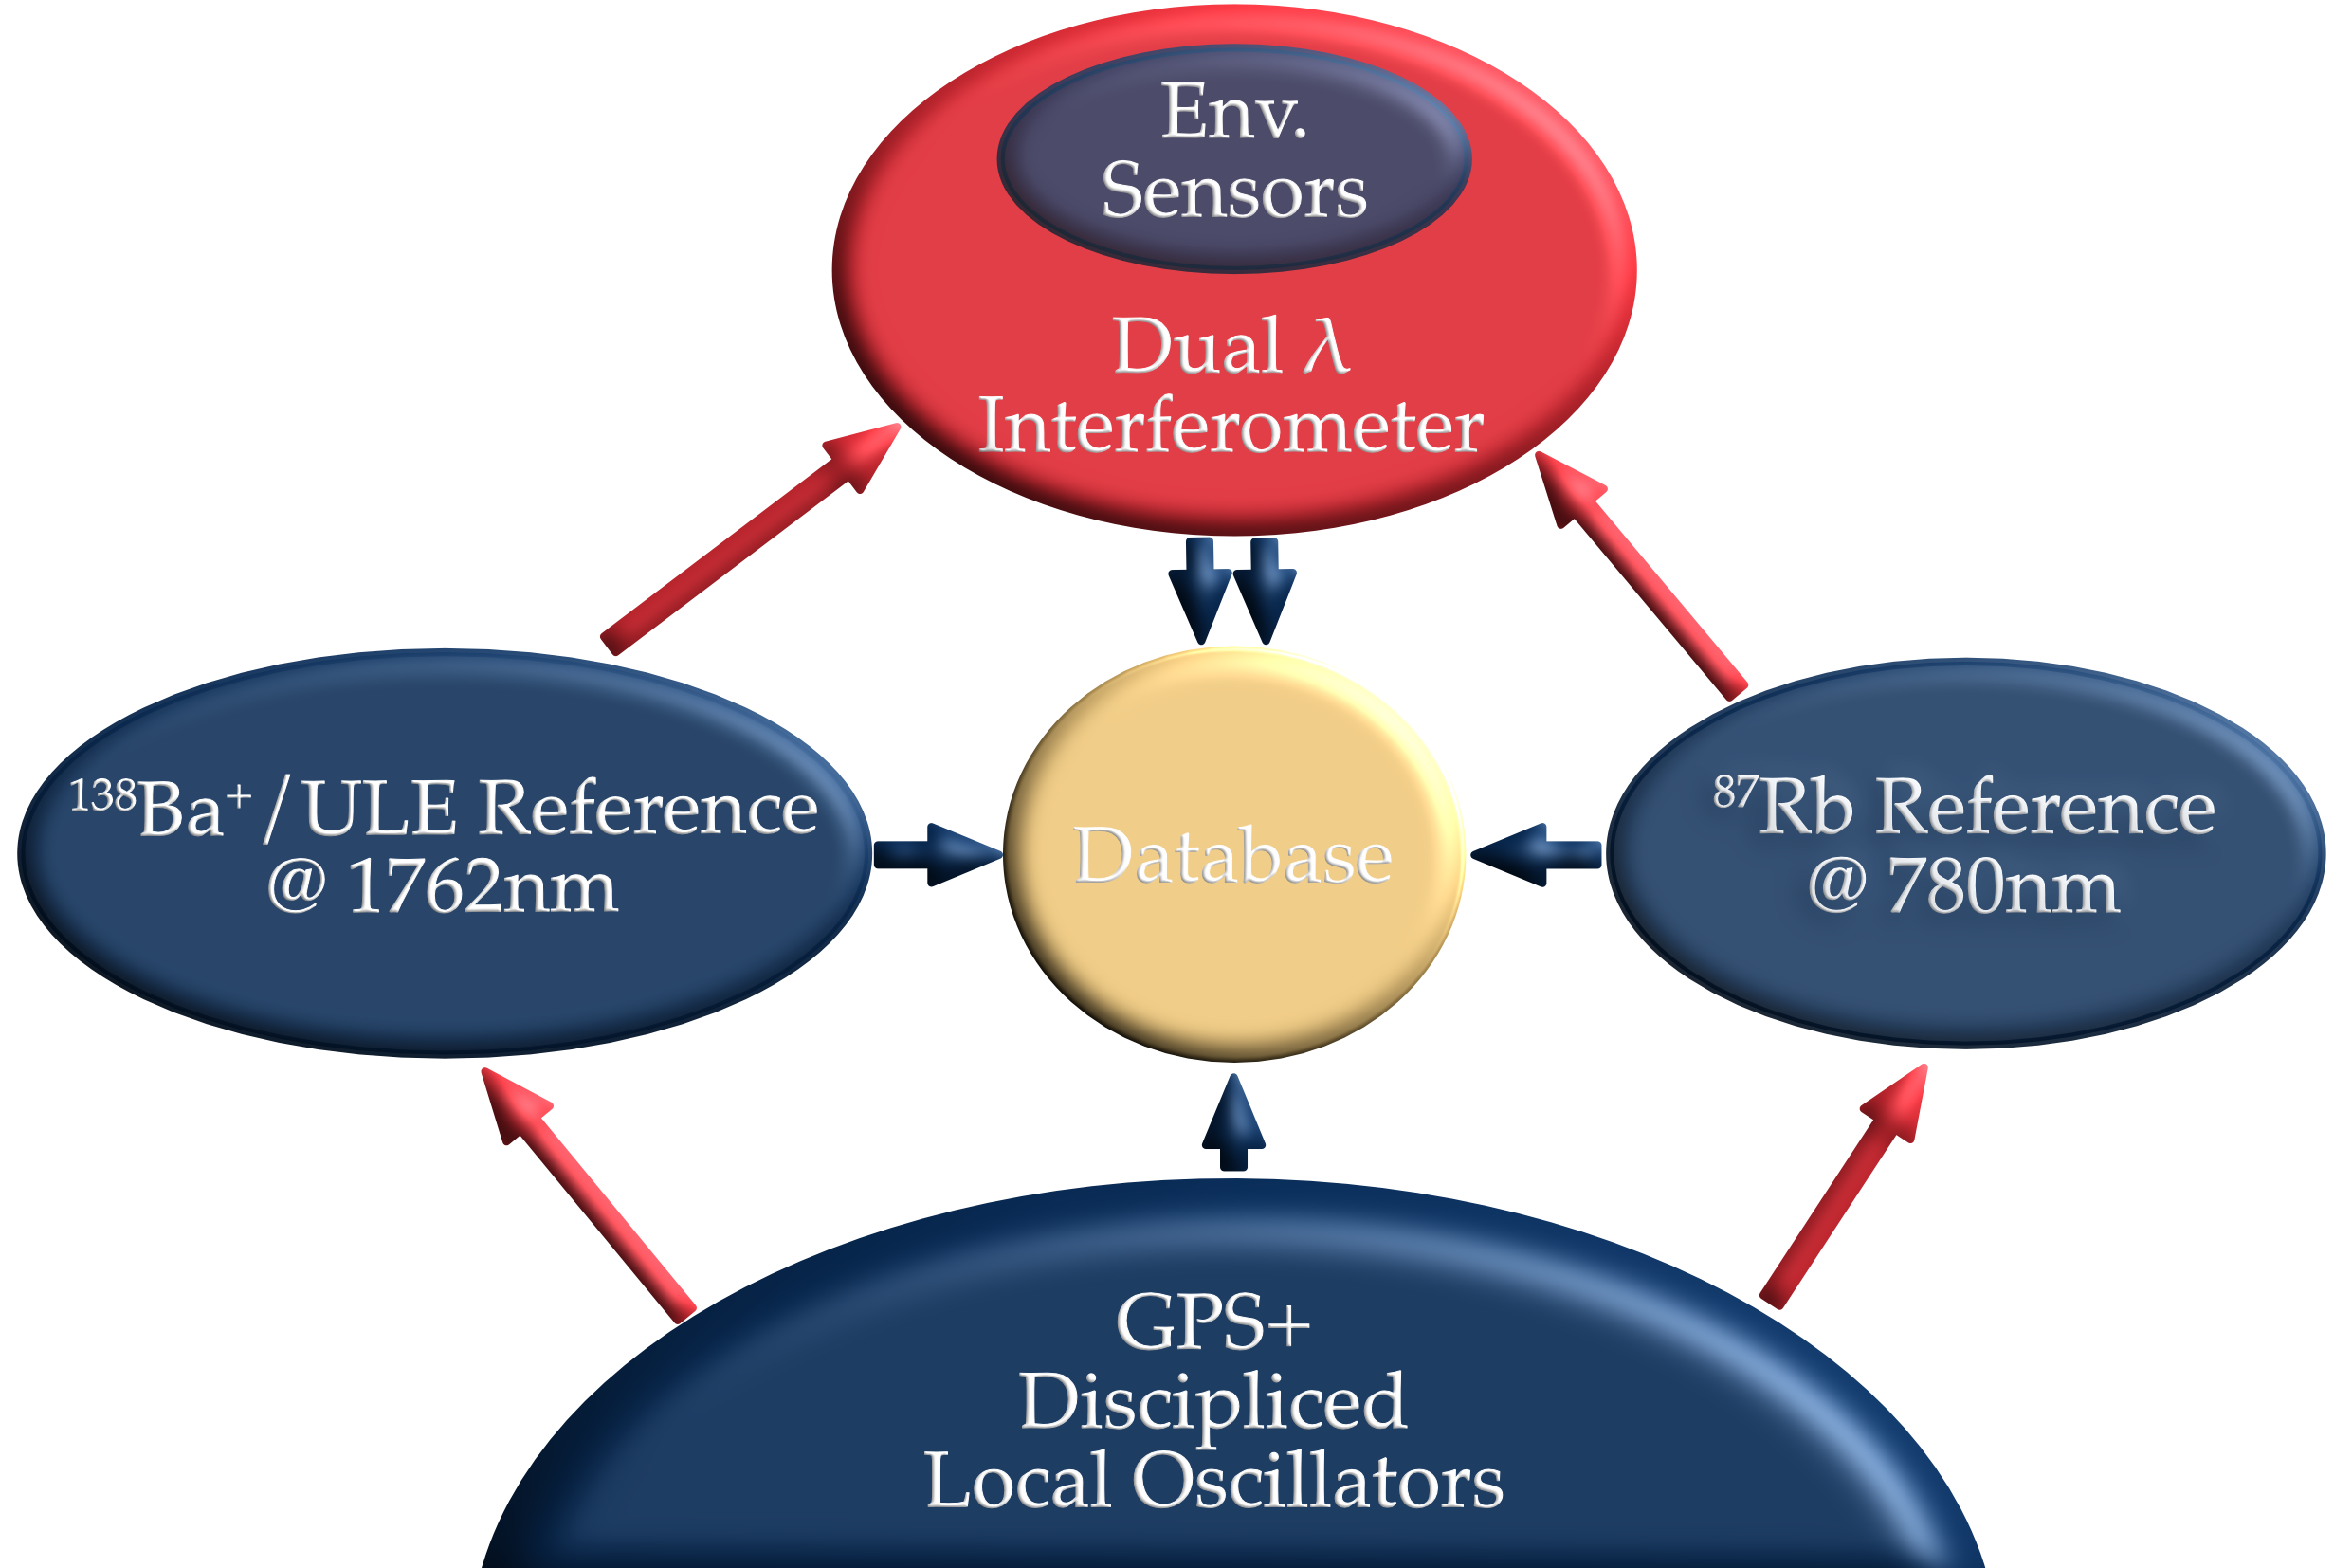
\includegraphics[width=0.45\textwidth]{figures/figure1_3d.png}
\caption{Schematic of the experimental setup for quantum-referenced precision refractometry.
\textbf{(Blue)} Measurement node: The \SI{1762}{\nano\meter} probe laser is stabilized to an ultra-low-expansion (ULE) optical cavity for short-term stability \cite{yum2017optical}, and then referenced to the electric quadrupole transition ($6S_{1/2} \rightarrow 5D_{5/2}$) of a single trapped $^{138}\mathrm{Ba}^+$ ion. This ion serves as an absolute quantum frequency reference, providing long-term stability and accuracy traceable to the atomic transition. The \SI{780}{\nano\meter} reference laser is stabilized via Doppler-free saturated absorption spectroscopy using a $^{87}$Rb vapor cell, representing a conventional atomic spectroscopic standard. A co-located BME280 sensor monitors temperature ($T$), humidity ($H$), and pressure ($P$) at the interferometer site. A global positioning system (GPS)-disciplined oscillator provides a \SI{10}{\mega\hertz} timebase for synchronization.
\textbf{(Red)} Interferometer node: A dual-wavelength Michelson interferometer is placed in a non-temperature-stabilized building corridor outside the laboratory in Freiburg, Germany. This location introduces slow environmental drifts and fluctuations (e.g., from daily temperature cycles) absent in a temperature-stabilized laboratory, allowing the study of refractive index changes under conditions analogous to field deployment.
\textbf{(Yellow)} Database: Correlates the dual-wavelength interferometer data with environmental sensor readings to establish precise refractive-index and phase relationships for feed-forward phase compensation in free-space quantum links.
}
\label{fig:architecture}
\end{figure}

\section{Experimental Methods}
\label{sec:methods}

The experimental system is organized into three functional blocks, color-coded in Fig.~\ref{fig:architecture}. The measurement node (blue) supplies the interferometer with phase-stable laser light and records environmental conditions: the \SI{1762}{\nano\meter} probe laser is referenced to a single trapped $^{138}\mathrm{Ba}^+$ ion, the \SI{780}{\nano\meter} reference laser is stabilized to the $^{87}$Rb D$_2$ line via Doppler-free saturated absorption spectroscopy ($\delta f < \SI{1}{\mega\hertz}$), and temperature, relative humidity (RH), and pressure are monitored by a co-located BME280 sensor (accuracy $\pm\SI{1.0}{\degreeCelsius}$, $\pm\SI{3}{\percent}$ RH, and $\pm\SI{1}{\hecto\pascal}$). Both lasers share a GPS-disciplined \SI{10}{\mega\hertz} timebase, which stamps all measurements for synchronization with the interferometer node (red) and the time-series database (yellow). Environmental sensors were sampled at \SI{2}{\hertz}; interferometer fringe counts, requiring 10--20~s per measurement, were synchronised to the same GPS-disciplined \SI{10}{\mega\hertz} timebase.

The \SI{1762}{\nano\meter} probe laser addresses the $6S_{1/2} \rightarrow 5D_{5/2}$ electric quadrupole transition of $^{138}\mathrm{Ba}^+$ \cite{arnold2020precision}. It is stabilized to an ultra-low-expansion (ULE) optical cavity (finesse 360,000), which is in turn referenced to a single trapped ion via electric quadrupole spectroscopy, yielding short-term stability $\delta f < \SI{1}{\kilo\hertz}$.

A dual-wavelength Michelson interferometer (modified NIST LM10) \cite{fox1999reliable}) measures the differential phase accumulation between the two different wavelengths over a \SI{4.2}{\meter} optical path. Simultaneous counting for interference fringes at both wavelengths provides robustness against common-mode mechanical vibrations, isolating the refractive-index-specific phase shifts of interest. The differential phase accumulated over the common round-trip optical path $L = \SI{4.2}{\meter}$ (total propagation) relates to the refractive indices at the two wavelengths as

\begin{equation}
\label{eqn:wavemeter}
\Delta\phi = 2\pi L\left(\frac{n_{1762}}{\lambda_{1762}} - \frac{n_{780}}{\lambda_{780}}\right)
\end{equation}

The Ciddor model is well validated at \SI{780}{\nano\meter} \cite{ciddor1996refractive} and provides $n_{780}$. Solving Eq.~(\ref{eqn:wavemeter}) for $n_{1762}$ then yields the time series of the refractive index at the probe wavelength; the calibration at \SI{1762}{\nano\meter} is therefore differential, anchored to that reference. The interferometer and one co-located BME280 environmental sensor \cite{bme280} are placed in a non-temperature-stabilized building corridor outside the laboratory, experiencing natural diurnal variations in temperature (\SIrange{15}{35}{\degreeCelsius}), relative humidity (\SIrange{20}{45}{\percent}), and pressure (\SIrange{965}{1000}{\hecto\pascal}). The quantum frequency references are operated in a temperature-stabilized laboratory, physically separating reference stability from environmental exposure. The complete dataset comprises \num{145784} synchronized measurements collected from January to August 2025 \cite{wu_2026_18800166}.

The refractive index at \SI{1762}{\nano\meter} is modeled as a linear function of the environmental variables,

\begin{equation}
n(T,H,P) = n_0 + \alpha_T T + \alpha_H H + \alpha_P P
\end{equation}

where $n_0$ is a fitted intercept and $\alpha_j$ are the environmental coefficients determined by multivariate ordinary least-squares (OLS) regression on the synchronized time series. Statistical robustness is validated through a suite of diagnostics detailed in Supplemental Material, including moving-block bootstrap resampling with a block length of 156 samples (twice the measured $1/e$ residual decorrelation time) and $B = 5000$ replications \cite{kunsch1989jackknife,politis1994stationary}, heteroskedasticity- and autocorrelation-consistent (HAC) standard errors with a Bartlett kernel matched to the same lag \cite{newey1987hypothesis,andrews1991heteroskedasticity} (agreeing with the bootstrap estimates within 3\%), and error-in-variables Monte Carlo propagation \cite{carroll2006measurement,fuller2009measurement}.

\begin{figure}[htbp]
\centering
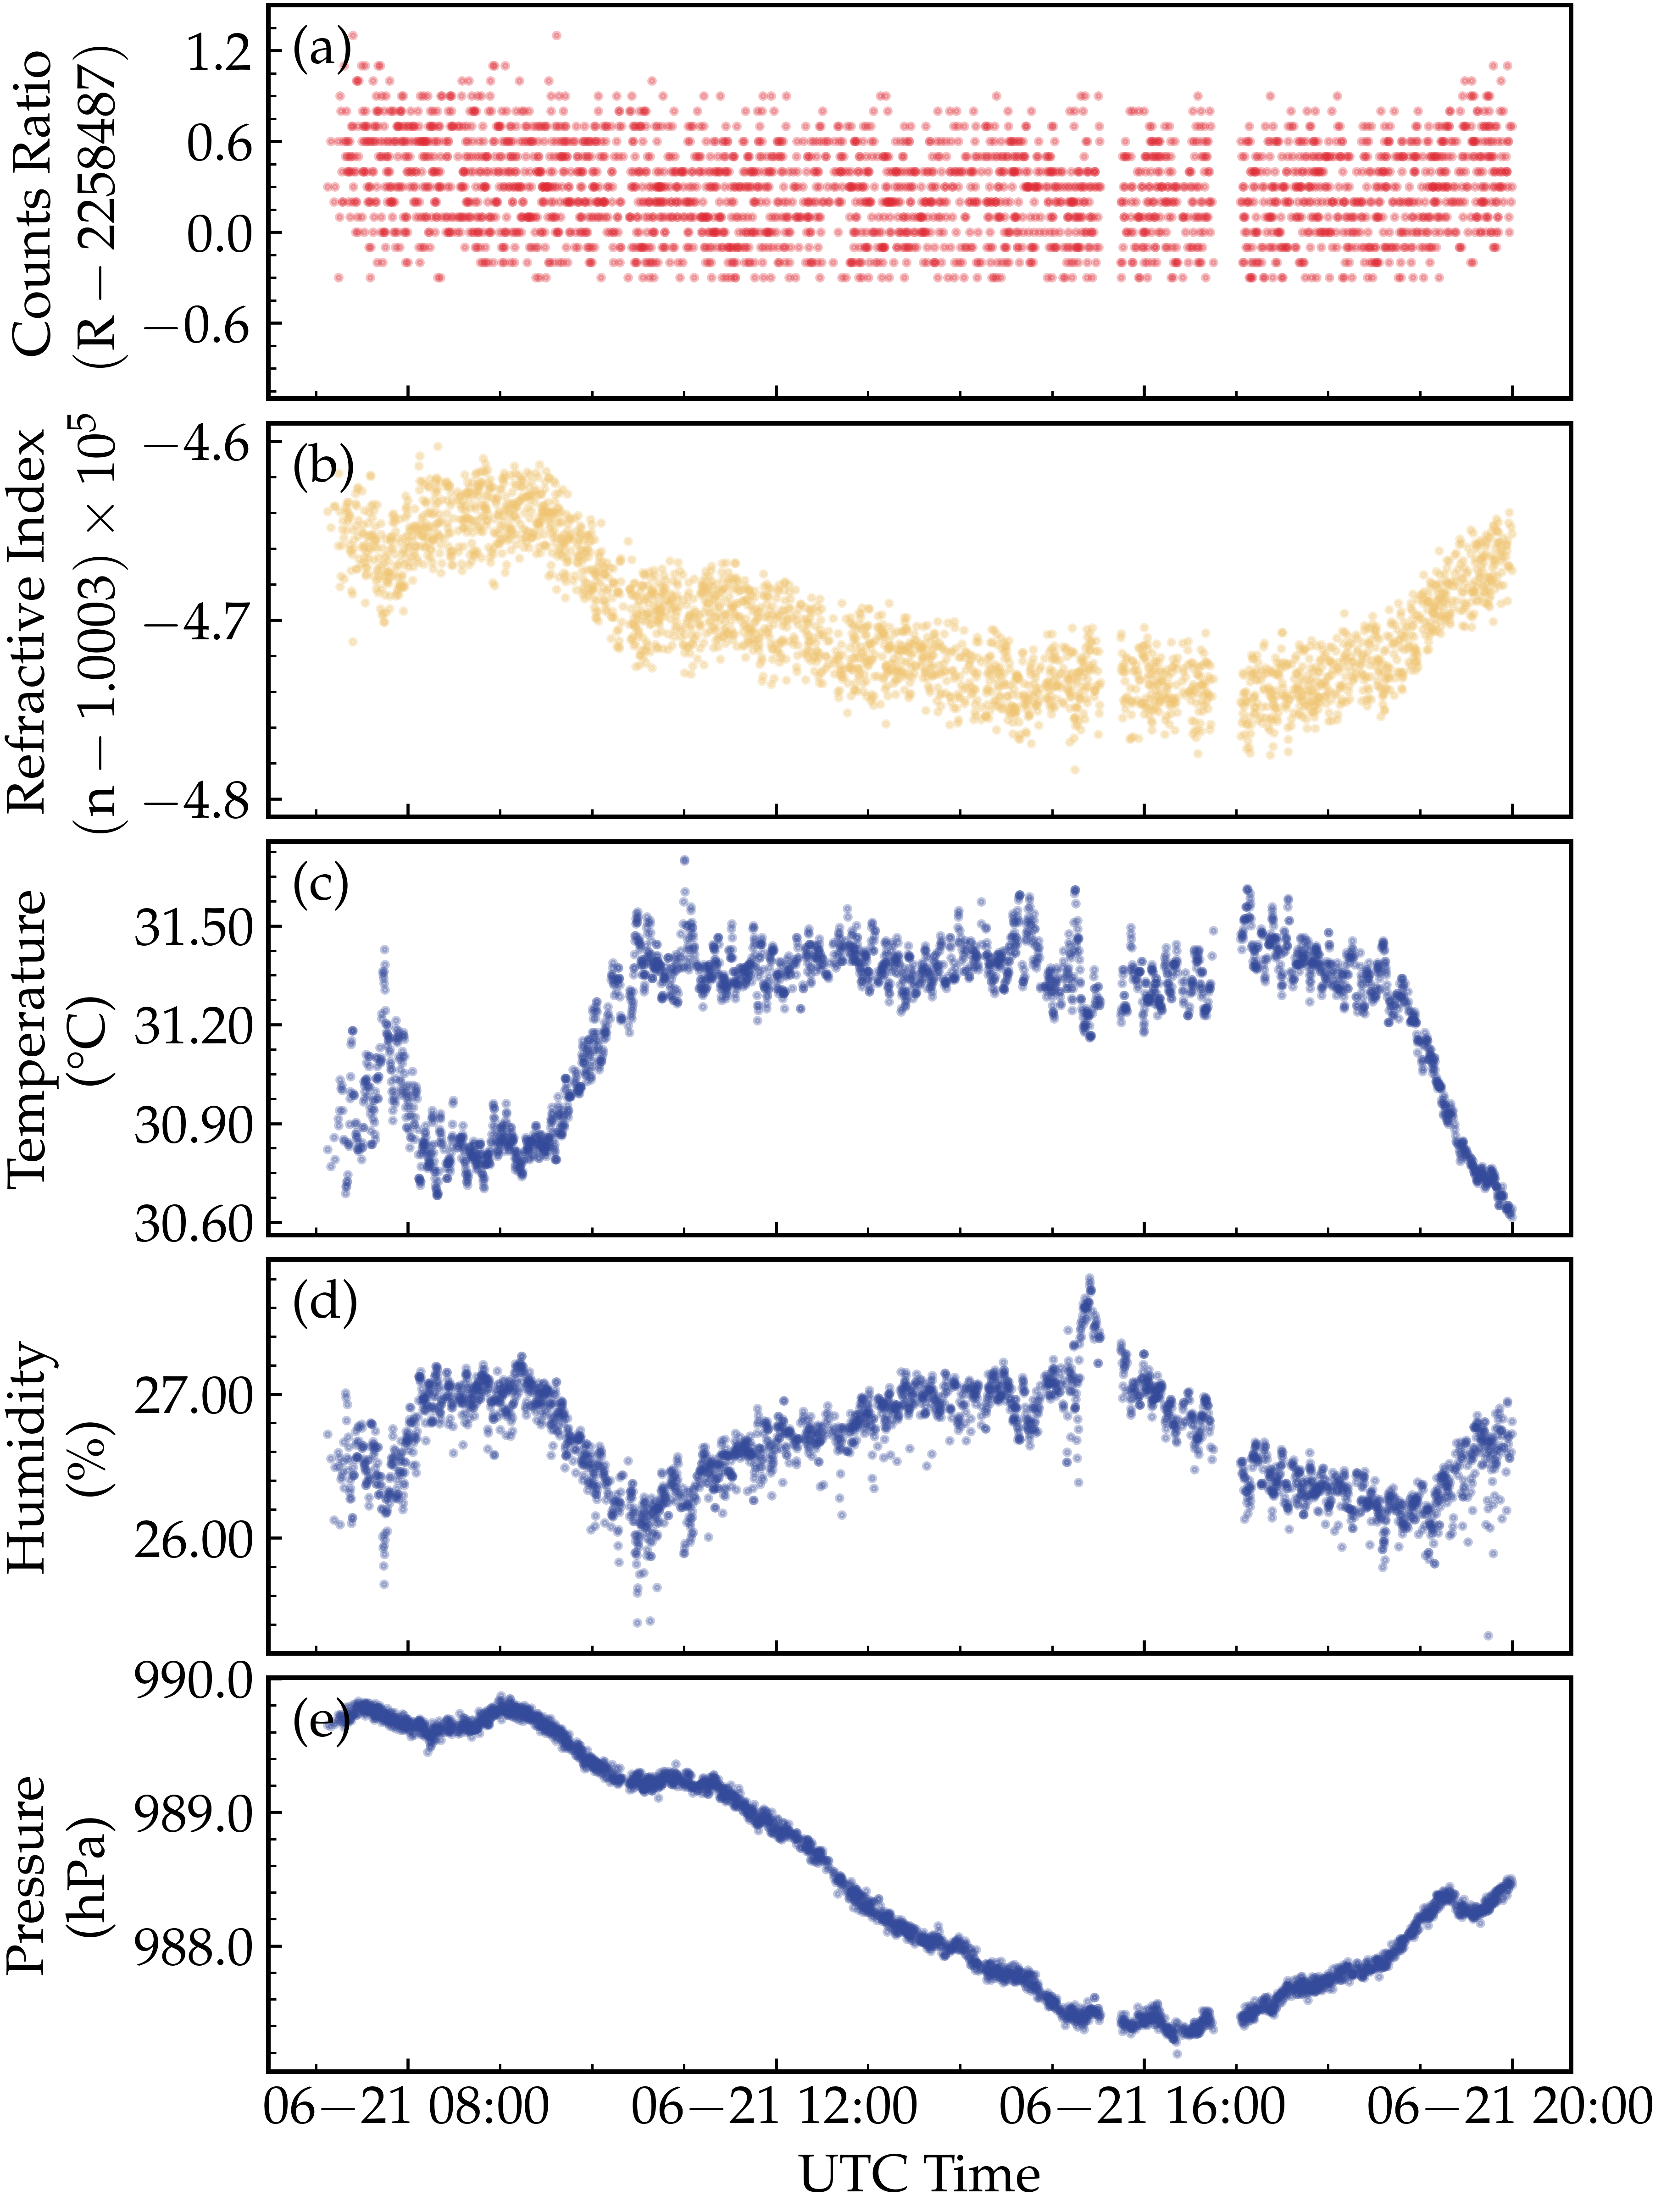
\includegraphics[width=0.45\textwidth]{figures/data_preview.png}
\caption{Synchronous measurement over a 14 h daytime period. \textbf{(a)} Normalised interference fringe contrast ratio from the dual-wavelength interferometer, used to extract the optical phase shift along the measurement path. \textbf{(b)} Refractive index derived from (a) via Eq.~(\ref{eqn:wavemeter}), referenced to the Ciddor model at 780 nm. \textbf{(c)} Ambient temperature, \textbf{(d)} relative humidity, and \textbf{(e)} pressure at the interferometer site, recorded by the co-located BME280. The diurnal anti-correlation between (c) and (d) is the physically expected behaviour. Gaps near 16:00 result from laser-unlock events.}
\label{fig:timeseries}
\end{figure}

\section{Results and Validation}
\label{sec:results}

The synchronized dataset of the derived refractive index and the related environmental parameters, shown in Fig.~\ref{fig:timeseries}, spans eight months of continuous operation with natural diurnal and seasonal variations. The mean temperature, relative humidity, and pressure over the measurement period are \SI{24.7}{\degreeCelsius}, \SI{31.2}{\percent}, and \SI{982.3}{\hecto\pascal}, with standard deviations of \SI{4.1}{\degreeCelsius}, \SI{5.8}{\percent}, and \SI{7.2}{\hecto\pascal}, respectively.

The refractive index time series, derived from differential phase accumulation between the \SI{1762}{\nano\meter} and \SI{780}{\nano\meter} interferometer channels, tracks the environmental fluctuations with clear diurnal periodicity. Data gaps, visible in Fig.~\ref{fig:timeseries}, result from ion reloading cycles and occasional interferometer realignment; all valid time points from the full dataset (Section~\ref{sec:methods}) are used for the regression analysis.

Multivariate regression following the linear model defined in Section~\ref{sec:methods} yields the environmental coefficients listed in Table~\ref{tab:coefficients}. To place the comparison with the Mathar model on equal footing, we evaluate the Mathar formulation at the identical $(T,H,P)$ rows of the campaign and fit the same linear surrogate model to both datasets, as detailed in Supplemental Material. The temperature and pressure coefficients agree with this same-condition Mathar surrogate within \SI{0.35}{\percent} and \SI{0.93}{\percent}, respectively. In contrast, the humidity coefficient differs by \SI{24.8}{\percent}, with the measured magnitude smaller than the surrogate. The humidity difference is statistically significant in the full campaign, but its direction is opposite to the enhancement expected from water-vapor dispersion, and the humidity-sensor gain systematic (Supplemental Material) spans the full observed difference; it is therefore reported as an unresolved systematic pending independent humidity sensor calibration.

\begin{table*}[htbp]
\centering
\caption{Measured and predicted environmental coefficients at
         \SI{1762}{\nano\meter}. Mathar surrogate values are obtained
         by fitting the same linear model to the Mathar formulation
         evaluated on the identical observed $(T,H,P)$ rows
         (Supplemental Material). Uncertainties are moving-block
         bootstrap standard errors ($B = 5000$, block length 156
         samples); systematic sensor contributions are provided in
         Supplemental Material.}
\label{tab:coefficients}
\begin{tabular}{lcccc}
\hline
Coefficient & This work & Mathar surrogate & Difference & $u_{\rm stat}$ \\
\hline
$\alpha_T$ (\si{K^{-1}})      & $-8.8474\times 10^{-7}$ & $-8.8164\times 10^{-7}$ & $-0.35\%$ & $1.42\times10^{-9}$ \\
$\alpha_H$ (\%RH$^{-1}$)      & $-1.3152\times 10^{-8}$ & $-1.7486\times 10^{-8}$ & $+24.8\%$ & $1.16\times10^{-9}$ \\
$\alpha_P$ (\si{hPa^{-1}})    & $+2.5949\times 10^{-7}$ & $+2.5710\times 10^{-7}$ & $+0.93\%$ & $9.95\times10^{-10}$ \\
\hline
\end{tabular}
\end{table*}

The proximity of \SI{1762}{\nano\meter} to water-vapor absorption features, with the two nearest H$_2$O lines at \SI{1761.0405}{\nano\meter} and \SI{1762.4852}{\nano\meter} \cite{gordon2022hitran2020}, motivates a Kramers-Kronig analysis of the expected humidity dispersion, detailed in Supplemental Material. The line-by-line prediction from the HITRAN2020 water-vapor spectrum yields a humidity coefficient of order $10^{-8}$\,\%RH$^{-1}$, close to the broadband Mathar formulation, i.e., no enhancement over the broadband model at this wavelength. This is consistent with the same-condition comparison above, where the measured humidity coefficient is found to be smaller in magnitude than the Mathar surrogate rather than enhanced. Given the unresolved sensor gain systematic, a quantitative attribution of the residual humidity difference to a wavelength-specific physical effect is not possible with the present data.

The environmental coefficients are converted to phase-shift sensitivity per unit environmental change for $L = \SI{1}{\meter}$ by multiplication with $2\pi L / \lambda$. The resulting engineering quantities are listed in Table~\ref{tab:phase_shift}.

\begin{table}[htbp]
\centering
\caption{Phase-shift sensitivities of free-space optical path per meter
         at \SI{1762}{\nano\meter}, derived from the measured environmental
         coefficients.}
\label{tab:phase_shift}
\begin{tabular}{lcc}
\hline
Environmental parameter & $\partial\phi/\partial X$ & Unit \\
\hline
Temperature          & 3.16  & \si{rad\,m^{-1}\,K^{-1}} \\
Relative humidity    & 0.047 & \si{rad\,m^{-1}\,(\%RH)^{-1}} \\
Pressure             & 0.93  & \si{rad\,m^{-1}\,hPa^{-1}} \\
\hline
\end{tabular}
\end{table}

These values allow for feed-forward phase compensation. For example, a \SI{1}{\degreeCelsius} temperature drift along \SI{1}{\meter} of uncontrolled optical path produces \SI{3.16}{\radian} of phase error. While the humidity sensitivity per unit remains smaller (\SI{0.047}{\radian} per \SI{1}{\percent} RH), daily humidity variations of \SIrange{10}{20}{\percent} in typical laboratory environments produce phase excursions of \SIrange{0.5}{0.9}{\radian}, comparable to temperature-driven effects under typical conditions.

The empirical model achieves a residual standard deviation $\sigma_n = 1.84 \times 10^{-7}$, corresponding to a coefficient of determination $R^2 = 0.996$. The Mathar formulation evaluated at the same wavelength produces a root-mean-square residual error of $1.18 \times 10^{-6}$, dominated by a static offset of \num{1.166e-6} (Fig.~\ref{fig:validation}(b)). Because this offset is constant over the campaign, a single baseline calibration, as a deployed system would perform, removes it, leaving a residual standard deviation of \num{1.93e-7}. On this offset-fair basis, the empirical model improves the residual phase error by \SI{4.9}{\percent} (amplitude) and \SI{9.5}{\percent} (variance) over the debiased Mathar model, consistent with the close coefficient agreement in Table~\ref{tab:coefficients}. This comparison, summarized in Fig.~\ref{fig:validation}, confirms that the Mathar model captures the environmental response at \SI{1762}{\nano\meter} to within the measurement noise after baseline calibration.

An expanded uncertainty budget is provided in Supplemental Material. The dominant contribution comes from the spatial and temporal mismatch between the environmental sensor and the optical path ($\delta n = 1.84 \times 10^{-7}$). The combined expanded uncertainty with coverage factor $k = 2$ is $3.68 \times 10^{-7}$, confirming that the empirical model's predictive accuracy is currently limited by the performance of the environmental sensors rather than by the laser frequency stability (contribution $\delta n < 10^{-12}$).

\begin{figure}[htbp]
\centering
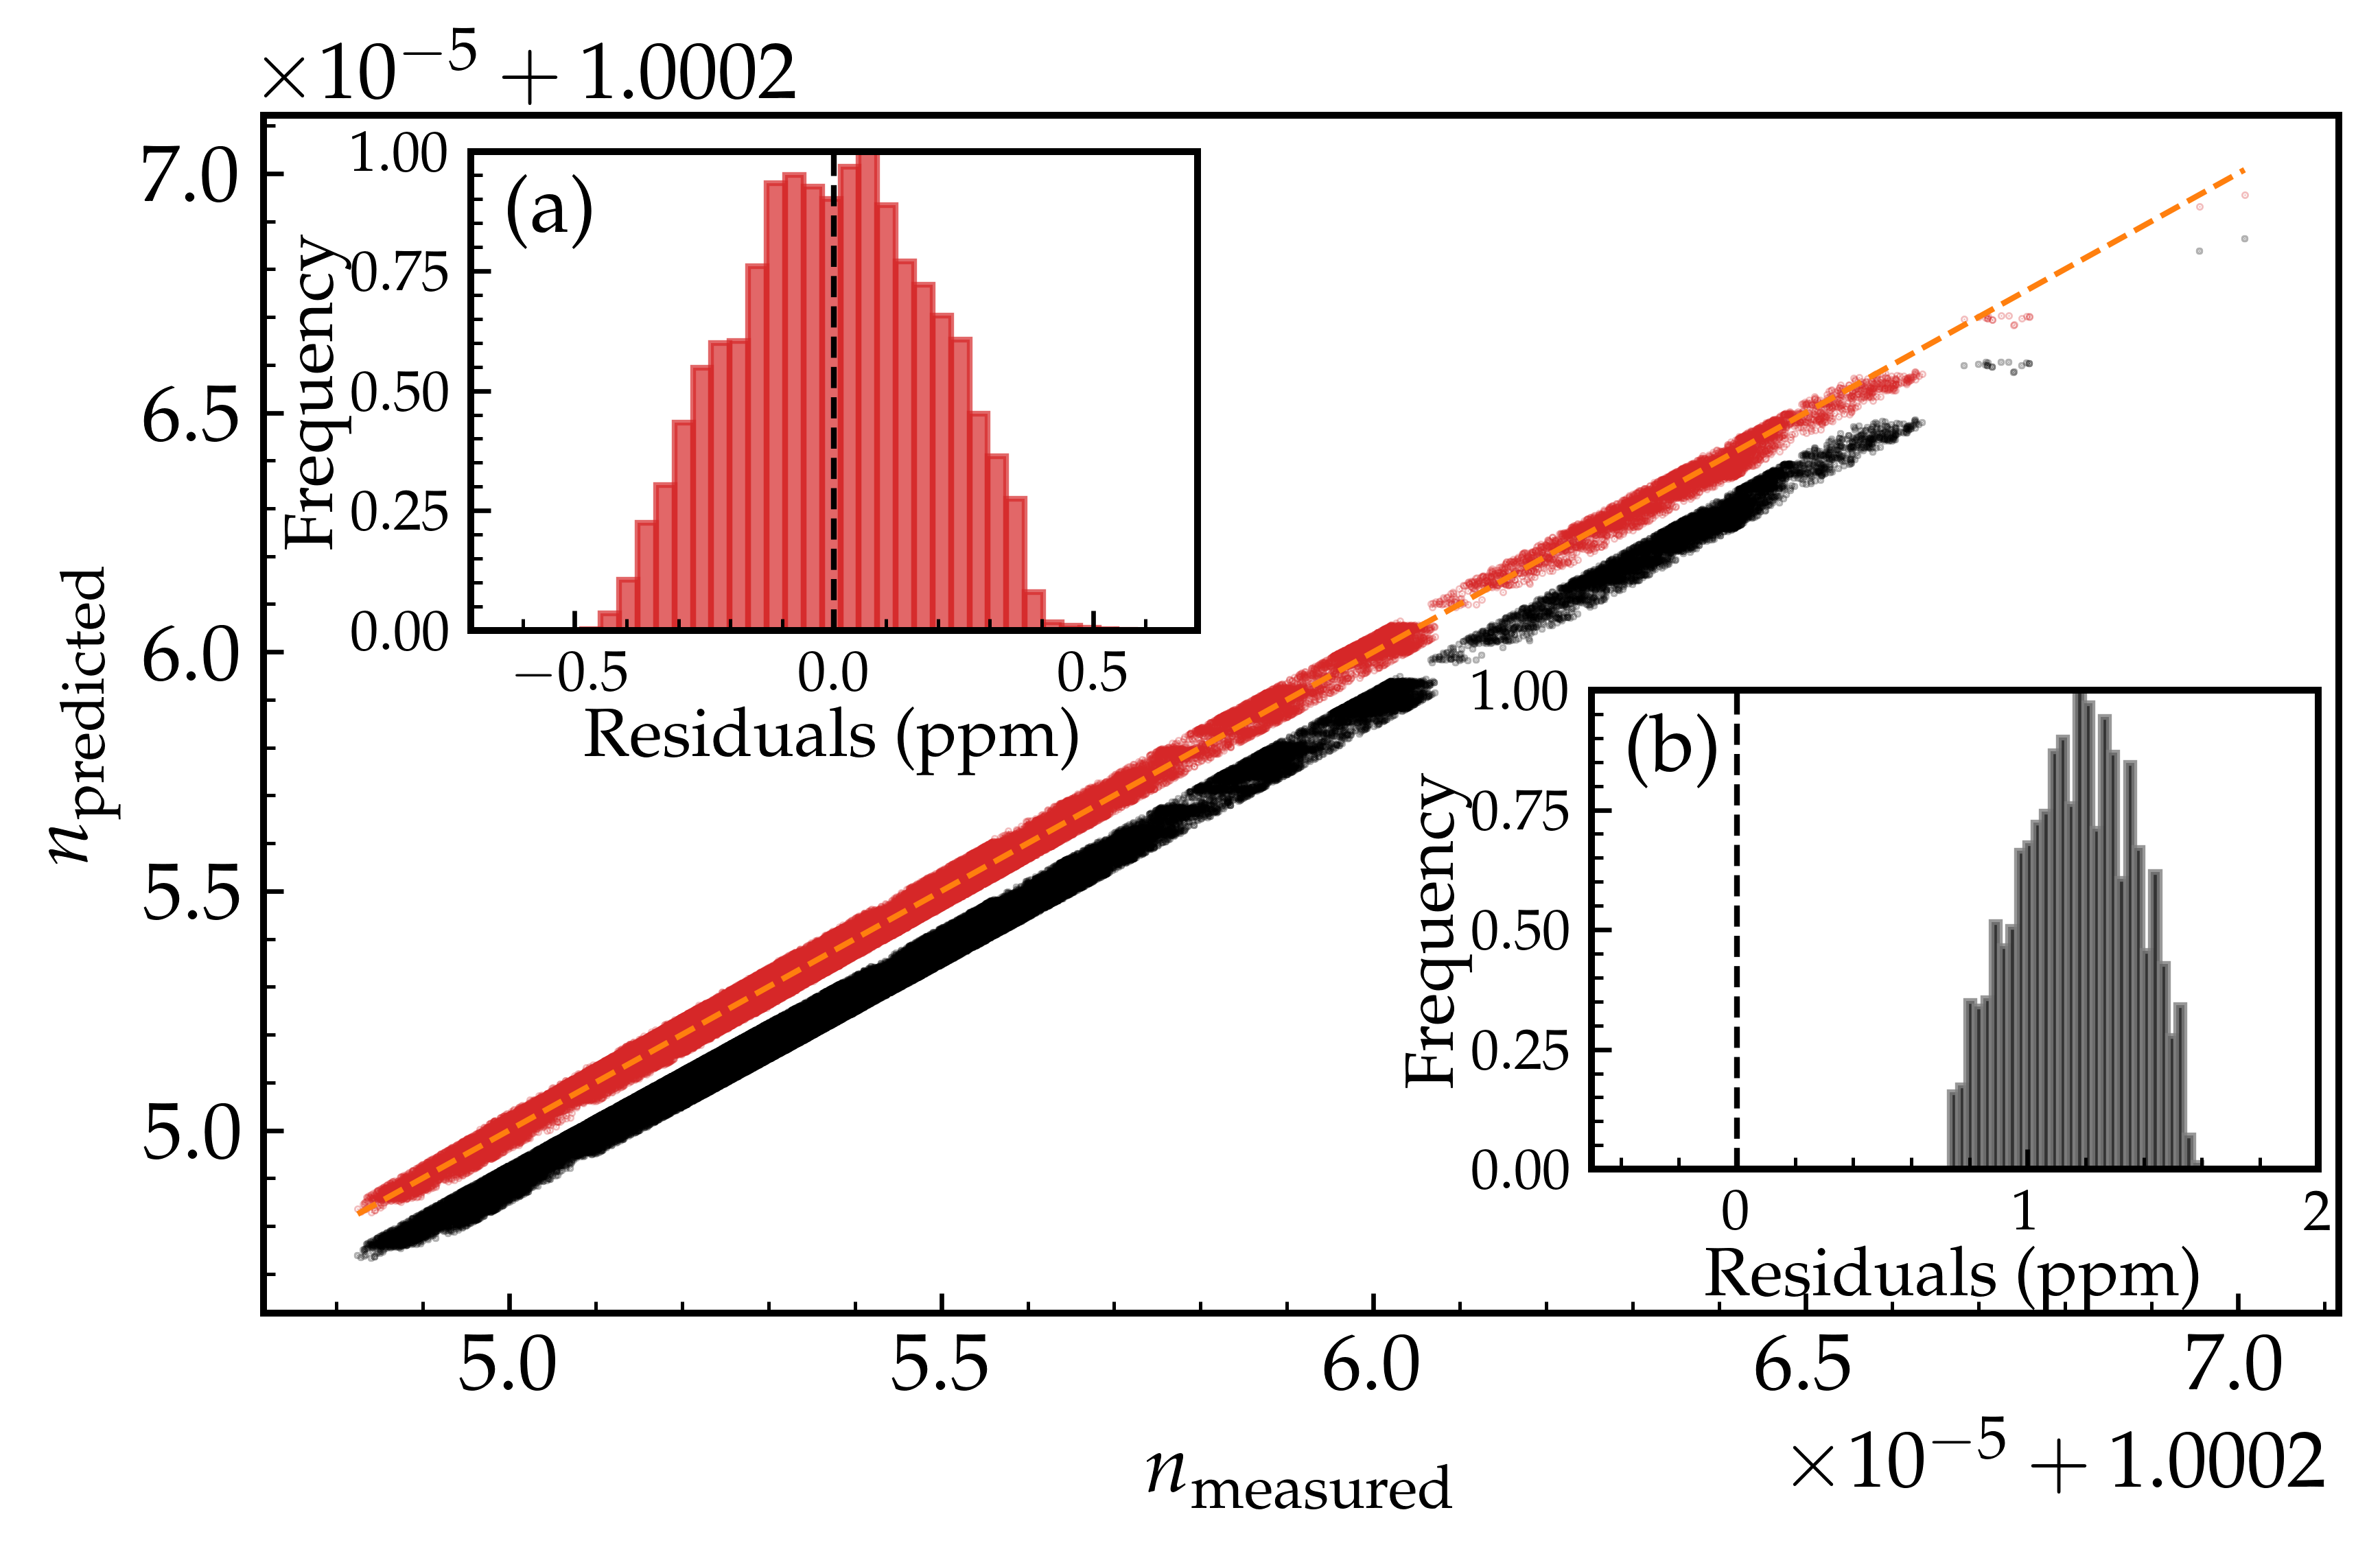
\includegraphics[width=0.45\textwidth]{figures/deviation_validation_with_full_data.png}
\caption{Validation of the empirical model for the refractive index of air at \SI{1762}{\nano\meter}. Main panel: Comparison of measured refractive index values with predictions from two models. Predictions from the empirical model developed in this work (red points) are compared against those from the published Mathar formulation \cite{mathar2007refractive} (black points, 1000-point subsample). The gold dashed line indicates the line of perfect agreement. The clustering of data points at higher and lower refractive index values corresponds to primary measurement campaigns conducted in winter and summer, respectively, with fewer measurements in intermediate conditions. \textbf{(a)} Residual distribution for the empirical model: mean \num{-2.802e-14}$\pm$\num{1.837e-07} standard deviation ($R^2 = 0.996$). \textbf{(b)} Residual distribution for the Mathar model: mean \num{1.166e-06}$\pm$\num{1.930e-07} standard deviation ($R^2 = 0.829$); the offset is a static calibration offset removable by a single baseline calibration, after which the residual standard deviation is \num{1.930e-07}, comparable to that of the empirical model.}
\label{fig:validation}
\end{figure}

\section{Discussion and Conclusion}
\label{sec:discussion}

The per-meter phase-shift sensitivities in Table~\ref{tab:phase_shift} apply directly to the free-space segments present in trapped-ion and neutral-atom quantum computing platforms. At every fiber-to-free-space transition, like fiber-to-vacuum-window coupling, acousto-optic modulator beamlines, and optical lattice projection optics, a short air path resides outside the temperature-stabilized enclosure. In a typical multi-beamline setup, these segments sum to \SIrange{0.5}{2}{\meter} and are subject to the same diurnal environmental swings studied here. For a representative \SI{1}{\meter} path under diurnal swings of $\Delta T = \SI{1}{\degreeCelsius}$, $\Delta H = \SI{12}{\percent}$, and $\Delta P = \SI{5}{\hecto\pascal}$, the total phase excursion exceeds \SI{5}{\radian} (detailed budget in Supplemental Material). A feed-forward correction using the measured coefficients reduces this to a residual of \SI{0.66}{\radian}. Compared with the Mathar model after a single baseline calibration (residual \SI{0.69}{\radian} per meter), the improvement is approximately \SI{5}{\percent}; the dominant raw Mathar residual arises from the static offset, which is removable by calibration. This estimate assumes the local environmental sensor reading remains representative of conditions along the optical path; deployment over longer baselines or through inhomogeneous air will require distributed sensing. With a \SI{10}{\minute} update interval between environmental sensor readings, the effective phase drift between corrections falls below \SI{0.03}{\radian}.

The coefficient comparison with the Mathar model has a practical consequence: broadband refractivity models capture the environmental response at \SI{1762}{\nano\meter} to within one percent for temperature and pressure after baseline calibration, while the humidity channel carries an unresolved, sensor-limited systematic. For quantum platforms, the linearity of the refractive index response and the close agreement with the Mathar model suggest that a modest library of empirically calibrated coefficients covering the principal species-specific transitions at \SI{729}{\nano\meter}, \SI{1762}{\nano\meter}, and \SI{2.1}{\micro\meter} would enable feed-forward compensation across all beamlines in a multi-species quantum computing platform. Factors that limit the achievable accuracy of the empirical model, as well as the inherent scope of what a single-point, slow-sampling feed-forward approach can correct in a deployed system, are discussed in Supplemental Material.

The same compensation strategy could extend to metropolitan-scale free-space quantum channels. At \SI{1762}{\nano\meter}, the native wavelength of the $^{138}\mathrm{Ba}^+$ qubit transition, a free-space channel spanning hundreds of meters under the diurnal swings considered here would accumulate a phase error on the order of $10^3$~\si{\radian} if uncorrected, which is sufficient to randomize the distributed entanglement entirely, a magnitude consistent with the phase-budget estimates for ground-level free-space entanglement distribution \cite{ursin2007entanglement}. Feed-forward compensation using the measured coefficients reduces this to a tractable residual, suggesting that atmospheric dispersion may be correctable rather than prohibitive for ground-level quantum network links. The methodology demonstrated here, pairing a quantum frequency reference with environmental monitoring for quantum-referenced refractometry, is transferable to free-space quantum channels operating at wavelengths where broadband refractive index models lack validation.

Beyond quantum networks, the per-meter phase-shift sensitivities in Table~\ref{tab:phase_shift} offer a direct pathway to improving systematic error budgets in precision optical metrology. In setups with multiple free-space beamlines, for example, individual addressing arrays, Raman sideband paths, or optical lattice projection optics, the cumulative phase budget benefits multiplicatively from per-wavelength compensation at each beamline. Beyond trapped ions, the methodology is applicable to precision optical measurements where uncompensated air dispersion forms a systematic error floor: long-baseline interferometry \cite{colavita2004effects,meiners2016overcoming}, optical clock comparisons over free-space links \cite{giorgetta2013optical,shen2022free}, and dimensional metrology. The empirical measurement at a target wavelength effectively converts the optical path into a refractometer of ambient air whose accuracy is set by the atomic frequency reference rather than by a proxy calibration chain. Viewed inversely, the same measurement configuration constitutes a quantum-referenced precision refractometer for atmospheric sensing, with potential relevance to distributed atmospheric refractometry and dimensional metrology.

The immediate extension is to replicate the measurement at other quantum-relevant wavelengths using either the same $^{138}\mathrm{Ba}^+$ clock or alternative atomic species. A library of empirically calibrated coefficients spanning \SI{400}{\nano\meter} to \SI{5}{\micro\meter} would enable feed-forward compensation across all optical beamlines in a multi-species quantum computing platform. Coupled with miniature environmental sensors integrated into the beamline enclosure, such a library would provide the basis for environmental phase compensation across multi-species quantum platforms. Longer-term, machine-learning surrogates trained on high-resolution HITRAN line lists \cite{gordon2022hitran2020} and validated by targeted empirical benchmarks as demonstrated here could generate continuous $\partial n/\partial X$ surfaces across wavelength, temperature, and humidity, providing a wavelength-resolved complement to the single-point broadband models currently embedded in quantum control software \cite{ukkonen2022improving}.

\begin{acknowledgments}
We thank F. Hasse, H. Bao, P. Mullan and D. Palani for fruitful discussions, as well as A. Windt and I. Zhuravlev for comments on the manuscript. This research was funded by the European Research Council (ERC) under the European Union's Horizon 2020 research and innovation programme (grant number 648330), the Deutsche Forschungsgemeinschaft (DFG, grant number SCHA 973/9-1-3017959) and the Georg H. Endress Foundation. W.W. acknowledges financial support from the QUSTEC programme, funded by the European Union's Horizon 2020 research and innovation programme under the Marie Sklodowska-Curie (grant number 847471). T.S. acknowledges financial support from the DFG via the RTG DYNCAM 2717 and the Georg H. Endress foundation.
\end{acknowledgments}

\section*{Data Availability}
The data that support the findings of this study, including the synchronized time series of interferometric phase measurements and co-located environmental sensor readings, are openly available on Zenodo at Ref.~\cite{wu_2026_18800166}. Analysis scripts used to perform the multivariate regression, statistical diagnostics, and Kramers-Kronig integration are included in the same repository.

\bibliography{reference}

\end{document}